\chapter{Implementacija i korisničko sučelje}
		
		
		\section{Korištene tehnologije i alati}
		
			 U svrhu ovog projekta korištene su sljedeće tehnologije i alati: Django i Bootstrap web programski okviri, sustav za upravljanje bazom podataka PostGreSQL, program pgAdmin, jezici HTML, CSS i JavaScript te biblioteku jQuery. \\
			 
			 
			 {Za pisanje backenda korišten je Django, web programski okvir utemeljen na jeziku Python. Preuzeti se može na ovoj  \href{https://www.djangoproject.com/}{\textbf{poveznici}}.
			 	
			 Baza podataka ostvarena je kroz sustav \href{https://www.postgresql.org/}{\textbf{PostGreSQL}} te uz pomoć programa \href{https://www.pgadmin.org/}{\textbf{pgAdmin}}.
			 
			 Frontend dio ostvaren je kroz korištenje standardnih jezika \href{https://www.w3schools.com/html/}{\textbf{HTML}},\href{https://www.w3schools.com/css/}{\textbf{CSS}} te \href{https://www.w3schools.com/js/DEFAULT.asp}{\textbf{JavaScript}}. Linkovi vode na stranice gdje se o njima može više saznati. 
			 
			 Uz navedene jezike korišteni su i programski okvir \href{https://getbootstrap.com/}{\textbf{Bootstrap}} pomoću kojeg su dobivene neke napredne funkcionalnosti frontenda te biblioteke \href{https://jquery.com/}{\textbf{jQuery}}.
			
			
			\eject 
		
	
		\section{Ispitivanje programskog rješenja}
			
			
			Ispitivanje se provodilo ručno. Kao temelj za ispitivanje koristili su se obrasci uporabe. Osim preciznog praćenja obrazaca također smo i nasumično navigirali po stranici u slučaju da negdje postoje greške u kodu (bugovi). Iako smo provjerili cijeli sustav radi pojednostavljenja u dokumentaciji prikazujemo samo 6 ispitnih slučajeva. Ispitali smo: UC2, UC3, UC10, UC18, UC20, UC24
			\\
			\\ 
			\textbf{Ispitni slučaj 1: Detaljan pregled priča}
			\\
			\textbf{Ulaz}
			\\
			\indent 1. Pritisak kursorom na određenu priču
			\\
			\textbf{Očekivani rezultat}
			\\
			\indent 1. Preusmjeravanje na stranicu odabrane priče
			\\
			\textbf{Rezultat}
			\\
			\indent Očekivani rezultat je zadovoljen te smo preusmjereni na stranicu za detaljan pregled priče koje smo odabrali. Slučaj je testiran i kao prijavljen korisnik i kao gost. Aplikacija je prošla test.
			\\ \\
			\begin{figure}[H]
				\centering
				\includegraphics[scale=0.34]{"slike/test1"}
				\caption{Rezultat ispitnog slučaja 1}
				\label{fig:rezultat-ispitnog-slucaja-1}
			\end{figure}
			
			\noindent \textbf{Ispitni slučaj 2: Komentiranje priče}
			\\
			\textbf{Ulaz}
			\\
			\indent 1. Navigacija do detaljnog pregleda priče \\
			\indent 2. Upisivanje samog komentara u predviđeno mjesto \\
			\indent 3. Pritisak gumba "Objavi"
			\\
			\textbf{Očekivani rezultat}
			\\
			\indent 1. Spremanje komentara u bazu za kasniji prikaz na stranici priče \\
			\indent 2. Osvježavanje stranice
			\\
			\textbf{Rezultat}
			\\
			\indent Očekivani rezultat je zadovoljen te se stranica osvježila te vidimo komentar koji smo ostavili. Komentar smo uspješno ostavili i kao gost i kao prijavljeni korisnik. Aplikacija je prošla test.
			\\ \\
			\begin{figure}[H]
				\centering
				\includegraphics[scale=0.34]{"slike/test2"}
				\caption{Rezultat ispitnog slučaja 2}
				\label{fig:rezultat-ispitnog-slucaja-2}
			\end{figure}
			
			\noindent \textbf{Ispitni slučaj 3: Predlaganje priče administratoru}
			\\
			\textbf{Ulaz}
			\\
			\indent 1. Navigacija stranice za prijedlog priče \\
			\indent 2. Odabir medije, naslova zahtjeva i naslova priče \\
			\indent 3. Pritisak gumba "Predloži priču"
			\\
			\textbf{Očekivani rezultat}
			\\
			\indent 1. Spremanje prijedloga priče u bazu \\
			\indent 2. Preusmjeravanje na stranicu sandučića
			\\
			\textbf{Rezultat}
			\\
			\indent Očekivani rezultat je zadovoljen. Preusmjereni smo na stranicu sandučića na kojoj vidimo još neobrađen zahtjev naše priče. Aplikacija je prošla test.
			\\ \\
			\begin{figure}[H]
				\centering
				\includegraphics[scale=0.34]{"slike/test3"}
				\caption{Rezultat ispitnog slučaja 3}
				\label{fig:rezultat-ispitnog-slucaja-3}
			\end{figure}
			
			\noindent \textbf{Ispitni slučaj 4: Pregled košarice}
			\\
			\textbf{Ulaz}
			\\
			\indent 1. Pritisak na gumb "Košarica" \\
			\textbf{Očekivani rezultat}
			\\
			\indent 1. Prikaz sadržaja u košarici, ukupne cijene te gumba za dovršavanje narudžbe. \\
			\textbf{Rezultat}
			\\
			\indent Očekivani rezultat je zadovoljen. Pritiskom na gumb košarica otvora se prikaz već navedenog sadržaja. Aplikacija je prošla test.
			\\ \\
			\begin{figure}[H]
				\centering
				\includegraphics[scale=0.34]{"slike/test4"}
				\caption{Rezultat ispitnog slučaja 4}
				\label{fig:rezultat-ispitnog-slucaja-4}
			\end{figure}
			
			\noindent \textbf{Ispitni slučaj 5: Promjena profilne slike}
			\\
			\textbf{Ulaz}
			\\
			\indent 1. Navigacija do stranice profila \\
			\indent 2. Odabir datoteke na računalu \\
			\indent 3. Pritisak gumba "Promijeni profilnu sliku" \\
			\textbf{Očekivani rezultat}
			\\
			\indent 1. Osvježavanje trenutne stranice na kojoj vidimo da je profilna slika promijenjena \\
			\textbf{Rezultat}
			\\
			\indent Očekivani rezultat nije zadovoljen. Namjerno nije odabrana nijedna slika, a gumb je svejedno pritisnut. Stranica se osvježila te profilna slika nije ažurirana.
			\\ \\
			\begin{figure}[H]
				\centering
				\includegraphics[scale=0.34]{"slike/test5"}
				\caption{Rezultat ispitnog slučaja 5}
				\label{fig:rezultat-ispitnog-slucaja-5}
			\end{figure}
			
			\noindent \textbf{Ispitni slučaj 6: Pregled registriranih korisnika}
			\\
			\textbf{Ulaz}
			\\
			\indent 1. Pritisak na ime korisnika bilo gdje na stranici \\
			\textbf{Očekivani rezultat}
			\\
			\indent 1. Prikaz profila odabranog korisnika. \\
			\textbf{Rezultat}
			\\
			\indent Očekivani rezultat je zadovoljen. Pritiskom na korisničko ime u komentarima preusmjereni smo na pregled profila odabranog korisnika. Aplikacija je prošla test.
			\\ \\
			\begin{figure}[H]
				\centering
				\includegraphics[scale=0.34]{"slike/test6"}
				\caption{Rezultat ispitnog slučaja 6}
				\label{fig:rezultat-ispitnog-slucaja-6}
			\end{figure}
			
			
			\subsection{Ispitivanje sustava}
			
			 \textit{Potrebno je provesti i opisati ispitivanje sustava koristeći radni okvir Selenium\footnote{\url{https://www.seleniumhq.org/}}. Razraditi \textbf{minimalno 4 ispitna slučaja} u kojima će se ispitati redovni slučajevi, rubni uvjeti te poziv funkcionalnosti koja nije implementirana/izaziva pogrešku kako bi se vidjelo na koji način sustav reagira kada nešto nije u potpunosti ostvareno. Ispitni slučaj se treba sastojati od ulaza (npr. korisničko ime i lozinka), očekivanog izlaza ili rezultata, koraka ispitivanja i dobivenog izlaza ili rezultata.\\ }
			 
			 \textit{Izradu ispitnih slučajeva pomoću radnog okvira Selenium moguće je provesti pomoću jednog od sljedeća dva alata:}
			 \begin{itemize}
			 	\item \textit{dodatak za preglednik \textbf{Selenium IDE} - snimanje korisnikovih akcija radi automatskog ponavljanja ispita	}
			 	\item \textit{\textbf{Selenium WebDriver} - podrška za pisanje ispita u jezicima Java, C\#, PHP koristeći posebno programsko sučelje.}
			 \end{itemize}
		 	\textit{Detalji o korištenju alata Selenium bit će prikazani na posebnom predavanju tijekom semestra.}
			
			\eject 
		
		
		\section{Dijagram razmještaja}
			
			Sustav je baziran na arhitekturi "klijent-poslužitelj". Koristimo HTTP za komunikaciju između korisnikovog uređaja i poslužitelja. Za posluživanje koristimo Heroku koji nudi platformu kao uslugu u oblaku. Heroku se sam brine o portovima, operativnim sustavima i okolinama poslužitelja pa nisu prikazani u dijagramu.
			
			\begin{figure}[!h]
				\centering
				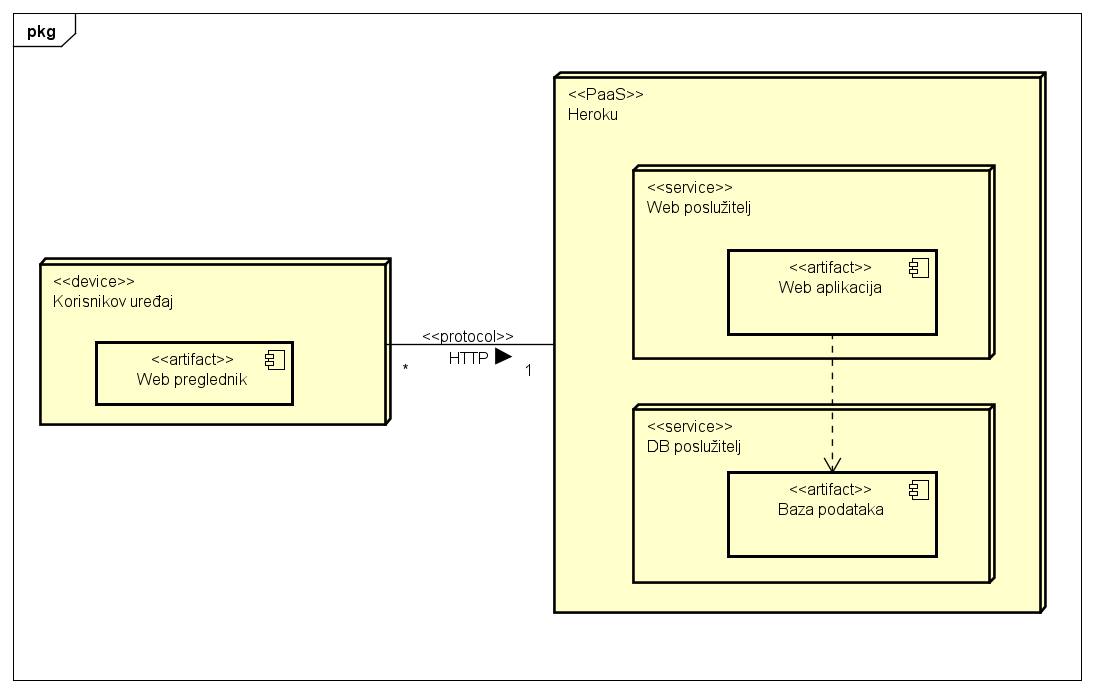
\includegraphics[width=1\linewidth]{slike/Dijagram_razmjestaja}
				\caption{Dijagram razmještaja}
				\label{fig:dijagramrazmjestaja}
			\end{figure}
			\eject
			
			\eject 
		
		\section{Upute za puštanje u pogon}
		
			\textbf{\textit{dio 2. revizije}}\\
		
			 \textit{U ovom poglavlju potrebno je dati upute za puštanje u pogon (engl. deployment) ostvarene aplikacije. Na primjer, za web aplikacije, opisati postupak kojim se od izvornog kôda dolazi do potpuno postavljene baze podataka i poslužitelja koji odgovara na upite korisnika. Za mobilnu aplikaciju, postupak kojim se aplikacija izgradi, te postavi na neku od trgovina. Za stolnu (engl. desktop) aplikaciju, postupak kojim se aplikacija instalira na računalo. Ukoliko mobilne i stolne aplikacije komuniciraju s poslužiteljem i/ili bazom podataka, opisati i postupak njihovog postavljanja. Pri izradi uputa preporučuje se \textbf{naglasiti korake instalacije uporabom natuknica} te koristiti što je više moguće \textbf{slike ekrana} (engl. screenshots) kako bi upute bile jasne i jednostavne za slijediti.}
			
			
			 \textit{Dovršenu aplikaciju potrebno je pokrenuti na javno dostupnom poslužitelju. Studentima se preporuča korištenje neke od sljedećih besplatnih usluga: \href{https://aws.amazon.com/}{Amazon AWS}, \href{https://azure.microsoft.com/en-us/}{Microsoft Azure} ili \href{https://www.heroku.com/}{Heroku}. Mobilne aplikacije trebaju biti objavljene na F-Droid, Google Play ili Amazon App trgovini.}
			
			
			\eject 